\documentclass[12pt]{article}
\usepackage{amsmath}
\usepackage{physics}

% Set border
\usepackage[margin=1in]{geometry}

% Use pictures and graphics
\usepackage{graphicx}
\graphicspath{ {images/} }

% Custom link colors
\usepackage{xcolor}
\usepackage{hyperref}
\hypersetup{
  colorlinks,
  linkcolor={black},
  citecolor={black},
  urlcolor={blue!80!black}
}

% Allow text to wrap around figures
\usepackage{wrapfig}

% Auto begin/end quotes (instead of having to use `` ")
\usepackage [autostyle, english = american]{csquotes}
\MakeOuterQuote{"}

% Used to include certain symbols (including /degree)
\usepackage{gensymb}

% TITLE ----------

\title{CMPU-250: Final Project Proposal \\
  \large Autonomous Robotics Design Competition Simulation}
\date{May 2018}
\author{George Witteman}

% DOCUMENT -------

\begin{document}

\maketitle

\section{Introduction}
For my project I'll be designing and implementing an agent-based model of Vassar's Autonomous Robotics Design Competition, and using the model to run simulations of runs of the competition using different parameters for how the robots move around the arena. 

I will simulate two robots competing for points using a modified version of the final competition rules taken from the course Moodle site.

\begin{wrapfigure}{O}[0.5in]{0.4\textwidth}
  \begin{center}
    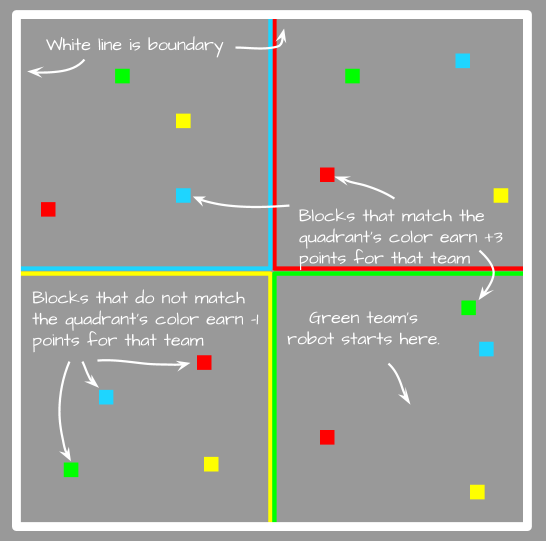
\includegraphics[width=0.35\textwidth]{arena.png}
  \end{center}
  \caption{Arena (without robots)}
  \label{fig:arena}
\end{wrapfigure}

\section{Rules of the (Simulated) Competition}

The following rules are adapted from the \href{https://docs.google.com/document/d/16FY8V81GwM7gtiwUqZmIOcLKY91lUuOmSKoWhPnytJs/edit}{original rules document}\footnote{\url{https://docs.google.com/document/d/16FY8V81GwM7gtiwUqZmIOcLKY91lUuOmSKoWhPnytJs/edit}}. Unless otherwise noted, the rules of this simulated competition are the same as the rules in the official rules document.

The competition arena consists of a grey square separated into four quadrants separated by a white boundary line. The four quadrants are delineated by red, green, blue, and yellow boundary lines, as shown in Figure \ref{fig:arena}. At the beginning of each round a red, green, blue, and yellow block is placed in each quadrant, for a total of twelve blocks on the arena. Two robots get placed in the middle of two random non-adjacent/opposite quadrants. For example one robot can start a round in blue and one in green, but one robot could not start in yellow and another in green. 

After five minutes has ended (i.e. a round has ended), teams earn three points for every block in their quadrant that matches their home quadrant color, and lose one point for every block that is not a match. The winner of the round is the team with the most points.

\section{What I'll Be Modeling}
My model will include the arena, four blocks of each color (red, blue, green, and yellow), and two robots. Each robot will have a width and a height (in inches) that are set by parameters. Each block will be one-and-a-half inches in length, width, and height and the boundary lines will be two inches in width. Since the physical arena is made up of twenty-five two foot squares, the virtual arena will be ten feet by ten feet in size.

Each robot will have a simulated "camera" that allows it to see blocks. The camera will have different variables that determine the maximum distance that it can see a block (\texttt{max\_view\_dist}) and the angle of view that it is able to see (\texttt{max\_view\_angle}).

In a given time step, robots can go forward or backward at a given velocity $V$ and rotate a given number of degrees $R$. A robot going straight will have $R = 0$, a robot going left will have $R < 0$, and a robot going right will have $R > 0$.

A robot will drive towards the nearest block of it's color that it is able to "see". If cannot see any blocks then it will drive straight until it either sees a block or hits a white boundary line. Whenever a robot hits a white boundary line it will rotate a random number of degrees between -180\degree\ (left) and 180\degree\ (right). 

If the front of a robot comes in contact with a block of it's color, the block then gets captured by the the robot and the robot holds the block in a "chamber" underneath itself. If the block is of a different color it get's ejected out one side of the robot in order to simulate the sorting mechanism used in our real robot.

After a certain number of minutes (the parameter \texttt{homing\_time}), if the robot enters it's home quadrant it will stop moving so that the blocks are in it's home quadrant by the end of the round. This is consistent with the robot that my team (Flappy McDoodle) used in the final competition.

\section{Motivation}
The central hypothesis that I wish to test with this model is that a better camera, that is one with a larger field of view, will have better performance than one with no camera or a camera with a small field of view. 

Another thing that I want to test is how often on average it would take a robot to end up back in it's home quadrant. For our robot in the real competition we gave the robot a conservative two minutes to get back home. That typically gave us over a minute just waiting in the home quadrant, so it would be interesting to see how consistent this is using a simulated environment.

\section{Time-Varying Dynamics}
I will model the rotation of the robot if it sees a block of it's home color as a differential equation in terms of time. Let $R_{max}$ be the maximum angle of rotation possible, $d_{max}$ be the maximum view angle for the camera on a given robot, and $d$ be the degrees off center that a block is seen. The equation for the change in rotation angle for a robot is
\begin{equation}
  \frac{dR}{dt} = R_{max}dt \times \frac{\sqrt{\abs{d}}}{\sqrt{d_{max}}} \times \frac{d}{\abs{d}}.
\end{equation}

The first term in this equation, $R_{max}dt$, sets the maximum value that the robot can turn in a given time step. The second term, $\sqrt{\abs{d}}/\sqrt{d_{max}}$, gets the proportion of the maximum angle of rotation that the robot will turn given the position of the block that the robot sees. Finally, the last term, $d/\abs{d}$, sets the sign for the rotation angle in order to turn the robot in the correct direction.

\section{Simplifying Assumptions}
In this model I will assume that all robots have the same features and have the same general strategy of determining movement, however the exact parameters they use to move may differ. I'm also assuming that it is more important to bring blocks into the home quadrant than removing other color blocks or putting other color blocks into your opponents home quadrant, so I'm deciding only to model the behavior that brings blocks into the home quadrant.

I'm also assuming that the robot cameras are perfectly accurate and have a perfect field of view. This is a strong assumption given the real outcome of the competition, but my assumption is that with enough time calibrating the cameras on the real robots that this is a reasonable assumption to make.

Another assumption is that robots have perfect motors that are able to stop the robot and get it to it's desired velocity immediately. Although this is not exactly accurate with the real robots, the robots were typically able to come to a full stop and speed up almost immediately, so I think that this is a fair assumption.

Finally, I am not modeling the sorting mechanism itself and I'm assuming the sorting is instant and perfect. That is, the sorting happens as soon as the robot comes into contact with a block and blocks never get stuck or categorized incorrectly. 

\end{document}